% ==========================================================
% 5. Requisitos do Sistema
% ==========================================================
\chapter{Requisitos do Sistema}
\label{cap:requisitos}

\section{Descrição do sistema e Motivação}
Será modelado e implementado um sistema Web para a gestão centralizada de membros, cômputo automatizado de horas de extensão, acompanhamento disciplinar e organização interna da Commit Júnior. A aplicação integrará cadastro de membros, cálculo de tempo de permanência, envio de relatórios aos coordenadores de curso via e-mail, controle de advertências com prazos de validade automáticos, diretório corporativo com filtros de equipe e calendário de reuniões.

A motivação para o uso do software fundamenta-se na superação das fragilidades decorrentes do uso disperso de planilhas do Google Sheets e páginas do Notion. A solução proposta assegura integridade relacional, rastreabilidade via trilhas de auditoria, proteção de dados civis sensíveis e eliminação de tarefas operacionais manuais das lideranças da empresa júnior.

\section{Requisitos funcionais}

\subsection{Descrição dos atores}

\begin{center}
\footnotesize
\begin{longtable}{|c|p{2.6cm}|p{5.0cm}|p{2.1cm}|p{2.2cm}|}
\hline
\textbf{Num.} & \textbf{Nome} & \textbf{Descrição} & \textbf{Frequência de Uso} & \textbf{Proficiência em Web} \\
\hline
\endfirsthead
\hline
\textbf{Num.} & \textbf{Nome} & \textbf{Descrição} & \textbf{Frequência de Uso} & \textbf{Proficiência em Web} \\
\hline
\endhead

1 & Administrador & Responsável por parametrizar taxas de horas, cadastrar membros e gerenciar ocorrências disciplinares e relatórios acadêmicos. & Diária & Alta \\
\hline

2 & Setor Jurídico & Responsável pela auditoria e validação de termos contratuais de voluntariado, desligamento e certificados de participação. & Semanal & Alta \\
\hline

3 & Líder de Área (Diretor / Gerente) & Responsável por acompanhar sua diretoria ou squad, registrar ocorrências de pontuação e publicar avisos setoriais. & Diária & Alta \\
\hline

4 & Membro (Assessor / Consultor) & Membro que acessa o diretório de contatos, verifica seu saldo de horas e advertências, submete contestações e agenda compromissos. & Diária & Alta \\
\hline
\end{longtable}
\end{center}

\subsection{Lista de funcionalidades}

Foi identificada a seguinte lista de funções para este produto:

\begin{center}
\footnotesize
\begin{longtable}{|c|c|p{3.1cm}|p{7.5cm}|}
\hline
\textbf{Cod} & \textbf{Tipo} & \textbf{Nome da função} & \textbf{Descrição} \\
\hline
\endfirsthead
\hline
\textbf{Cod} & \textbf{Tipo} & \textbf{Nome da função} & \textbf{Descrição} \\
\hline
\endhead

UC-01 & 3 & Login e Autenticação & Validação de acesso por meio de e-mail institucional e credencial criptografada, atribuindo perfil de permissão compatível. \\
\hline

UC-02 & 1 & Gerenciar Cadastro de Membros & Cadastro, alteração cadastral e exclusão lógica de dados civis (CPF, RG, endereço), acadêmicos (matrícula, campus, curso) e organizacionais (cargo, diretoria, área, GitHub). \\
\hline

UC-03 & 1 & Gerenciar Documentação e Termos & Acompanhamento de conformidade de assinatura dos Termos de Voluntariado, Termos de Desligamento e Certificados de Extensão. \\
\hline

UC-04 & 1 & Parametrizar Regras de Horas & Configuração da carga horária de extensão conferida por período a cada cargo e função ocupada no organograma. \\
\hline

UC-05 & 2 & Contabilizar Horas de Extensão e Tempo de Casa & Processamento do somatório de horas de extensão com base nas datas de exercício das funções e cômputo da senioridade institucional do membro. \\
\hline

UC-06 & 4 & Notificar e Enviar Horas para a Coordenação & Agrupamento dos totais de horas aprovadas e despacho formal via correio eletrônico institucional à coordenação responsável pelo registro no SIGAA. \\
\hline

UC-07 & 1 & Gerenciar Pontos e Penalidades & Registro de infrações disciplinares com pontuação associada, cálculo automático de validade de expiração e incidência de agravantes de reincidência. \\
\hline

UC-08 & 1 & Contestar Pontuações & Submissão de justificativa formal pelo membro contra pontuações recebidas, retendo o status como pendente até julgamento da diretoria. \\
\hline

UC-09 & 2 & Exibir Diretório de Equipe e Rankings & Painel de membros ativos filtrados por campus, diretoria e squad, com indicadores consolidados de horas e engajamento por área. \\
\hline

UC-10 & 1 & Gerenciar Quadro de Avisos & Publicação e consulta de notas informativas direcionadas a toda a instituição ou restritas a áreas específicas. \\
\hline

UC-11 & 1 & Gerenciar Calendário e Agendamento & Gestão de eventos corporativos (Reuniões Gerais e treinamentos) e agendamento de reuniões individuais (1-on-1) com verificação de choque de horário. \\
\hline
\end{longtable}
\end{center}

{\footnotesize
\noindent\textbf{Tipo:} 1 -- Cadastro (Entrada) \hfill 2 -- Relatório (Saída) \hfill 3 -- Controle de Acesso \hfill 4 -- Outro\par}

% Limpa os elementos pendentes para iniciar o DCU sem acúmulo de tabelas
\clearpage

\subsection{Diagrama de casos de uso (DCU)}

Link para o DCU: \url{https://drive.google.com/file/d/1It3V4zqqA9LMgIkKsWDLE538FDhiWksD/view?usp=sharing}

\begin{figure}[!htbp]
    \centering
    \caption[Diagrama de Casos de Uso do SIGEJ]{Diagrama de Casos de Uso do Sistema Integrado de Gestão de Empresa Júnior (SIGEJ) da Commit Júnior}
    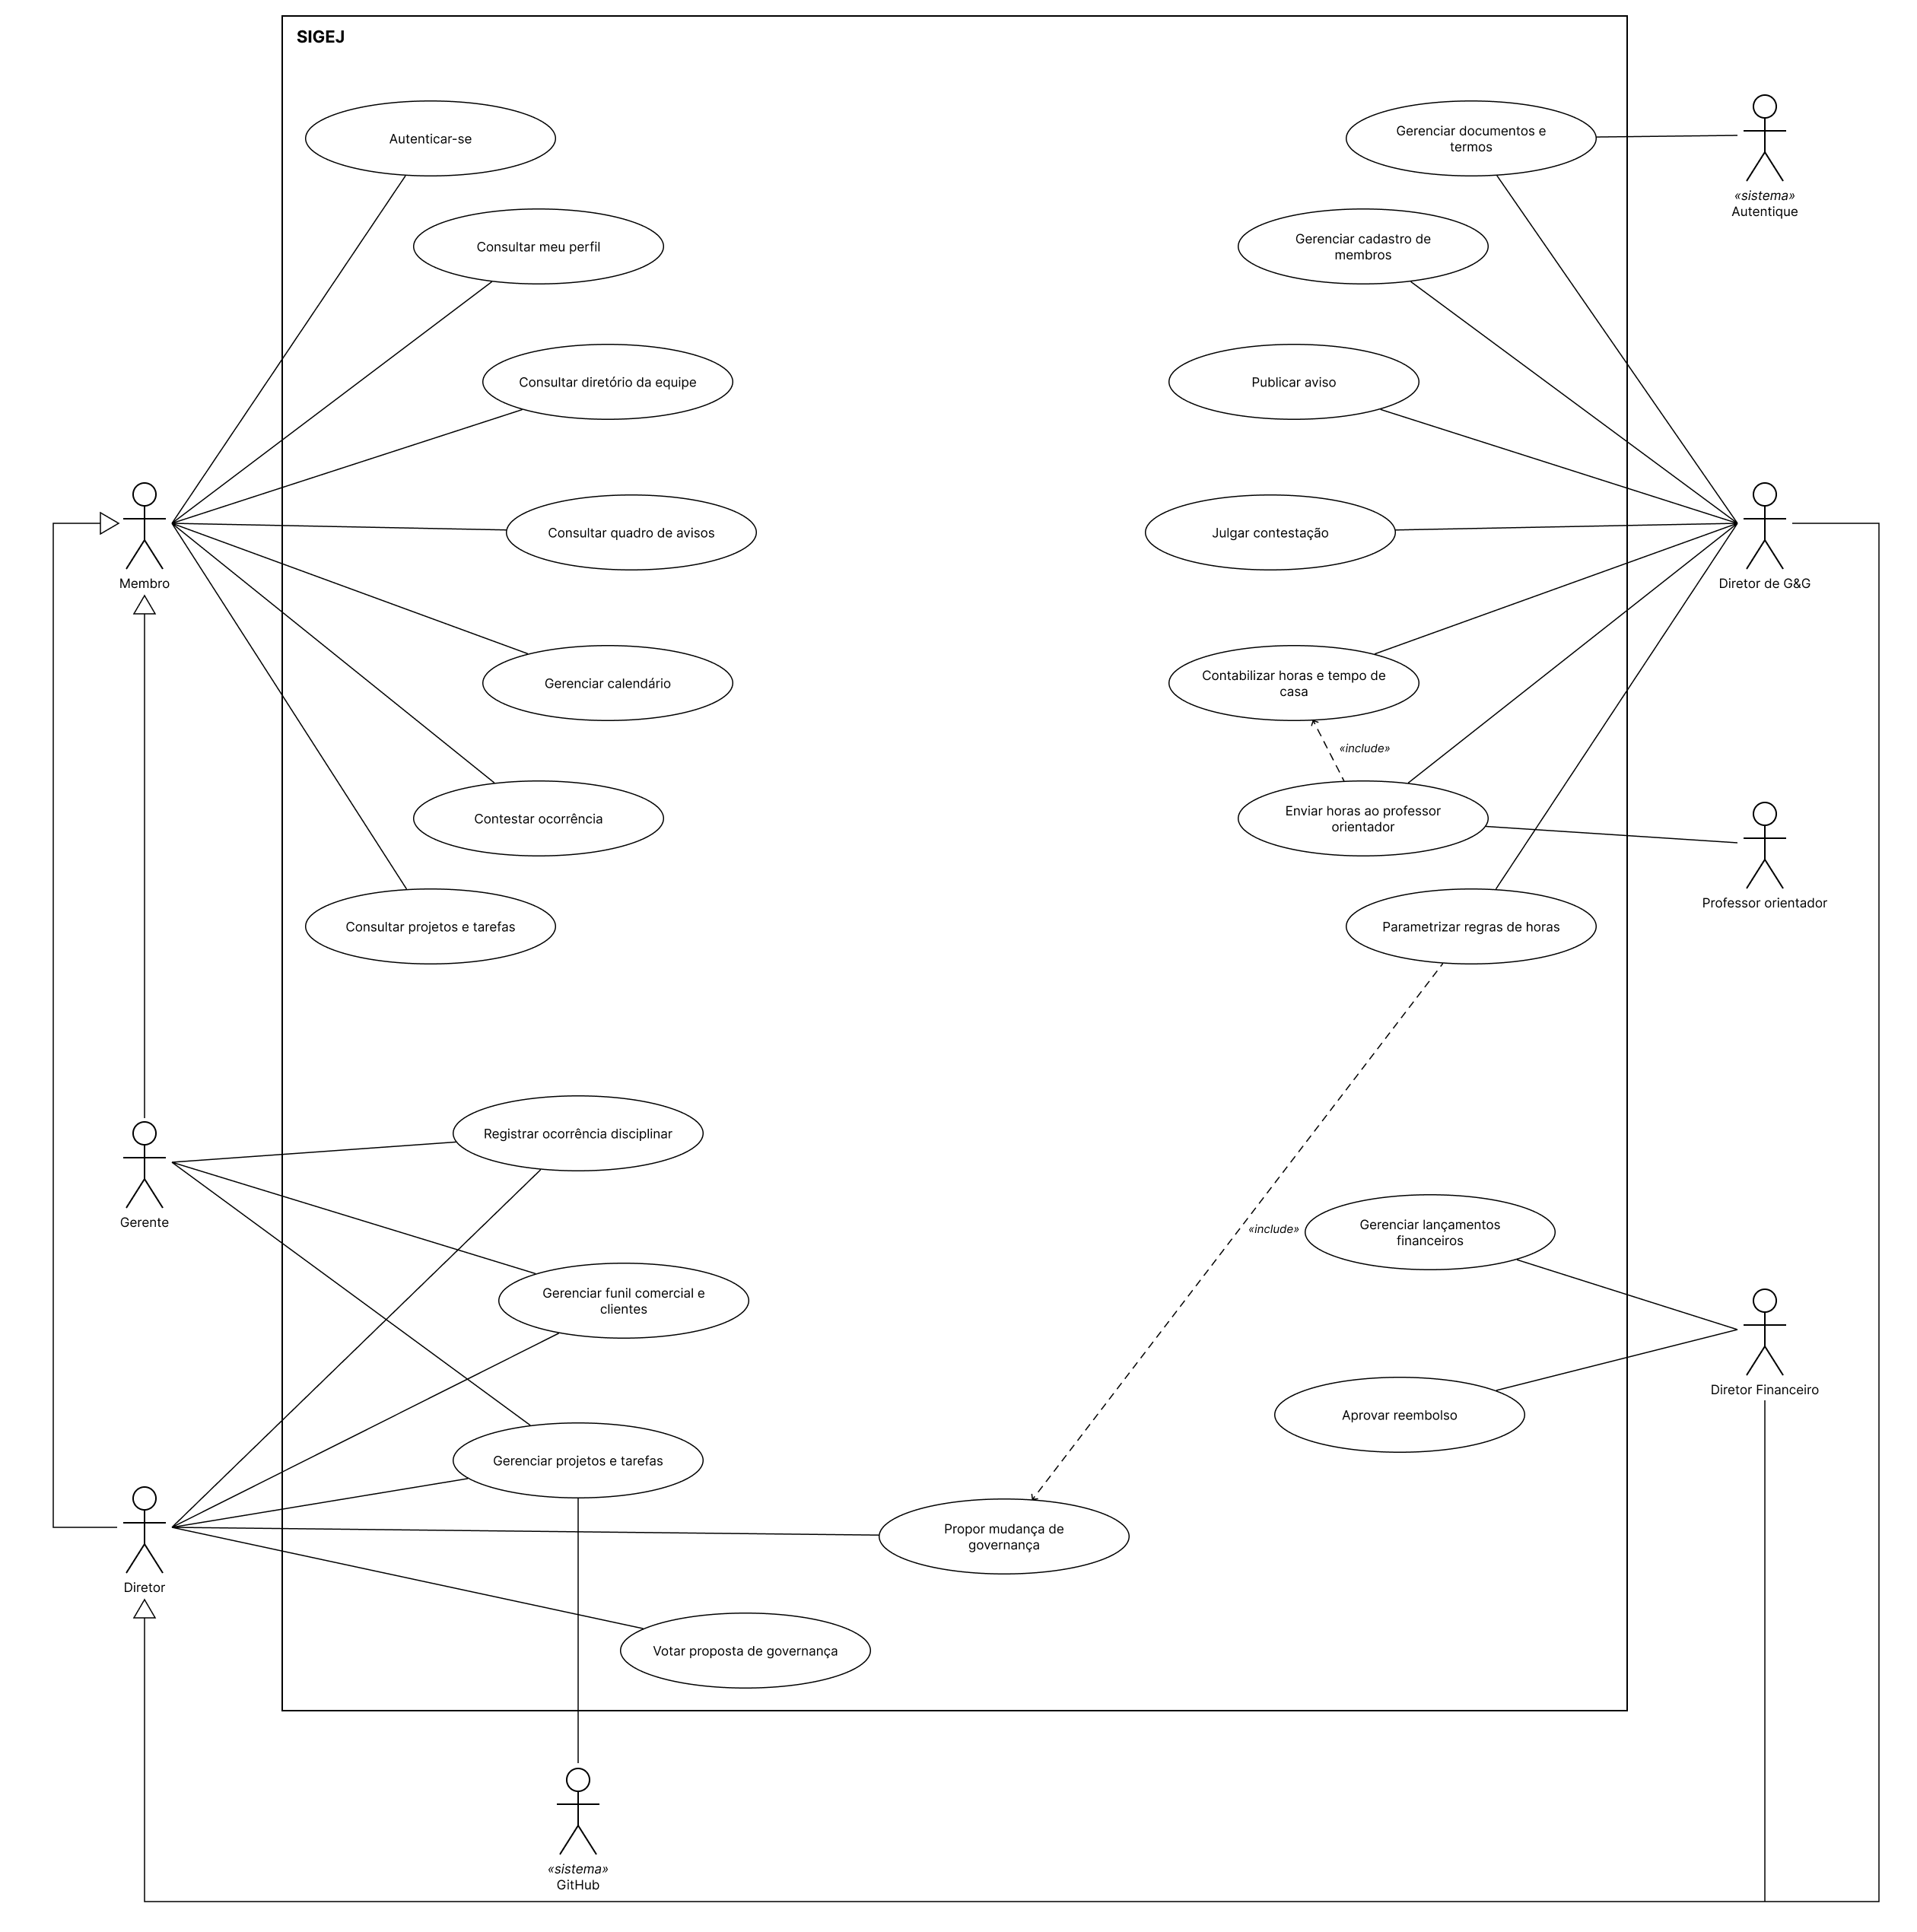
\includegraphics[width=0.9\textwidth,height=0.7\textheight,keepaspectratio]{diagrama.png}
    \label{fig:dcu-commit}
\end{figure}

% Bloqueia estritamente a descida da imagem para as seções abaixo
\clearpage

\subsection{Regras do negócio}

\textbf{RN01 - Unicidade Cadastral}: Todo integrante deve possuir identificação única no banco de dados referenciada por seu CPF e número de matrícula acadêmica.

\textbf{RN02 - Cômputo Proporcional de Horas}: As horas de extensão são computadas diretamente multiplicando o intervalo de tempo de permanência no cargo pela taxa horária previamente homologada para a função.

\textbf{RN03 - Preservação Histórica e Desativação Lógica}: Membros vinculados a horas, pontos, termos ou eventos institucionais não sofrem exclusão física; sua inativação deve ser efetuada via alteração para status ``Desligado'' ou ``Alumnus''.

\textbf{RN04 - Visibilidade Restrita a Membros Ativos}: O diretório geral de consulta corporativa deve exibir somente os integrantes com vínculo ativo, ficando os registros históricos restritos à consulta das diretorias de Gestão de Pessoas e Jurídico.

\textbf{RN05 - Caducidade e Agravamento de Penalidades}: Toda ocorrência disciplinar possui data de validade definida no ato de lançamento; reincidências ocorridas dentro do prazo de vigência acarretam a incidência do multiplicador agravante automático.

\textbf{RN06 - Incompatibilidade de Agendamentos}: O sistema deve impedir a confirmação de reuniões individuais caso um dos participantes conste como confirmado em outro compromisso formal ou Reunião Geral no mesmo horário.

\subsection{Descrição dos Casos de Uso}

\begin{casodeuso}
\textbf{UC-01 - Login e Autenticação}

\textbf{Sumário:} Usuário informa suas credenciais para autenticar-se na plataforma.

\textbf{Ator Primário:} Membro, Líder de Área, Jurídico ou Administrador.

\textbf{Pré-condições:} Usuário previamente cadastrado e com status ativo no banco de dados.

\textbf{Fluxo Principal}

\noindent 1. Usuário acessa o sistema web.\\
2. Usuário fornece e-mail institucional e senha de acesso.\\
3. Sistema valida as credenciais contra a base autenticada.\\
4. Sistema inicia a sessão do usuário e direciona para o painel de seu perfil.

\textbf{Fluxo de Exceção (1):} Credenciais Inválidas
\begin{itemize}
    \item a. Sistema informa divergência de credenciais e convida o usuário a repetir a tentativa.
\end{itemize}

\textbf{Pós-condições:} Usuário autenticado na aplicação com perfil e níveis de acesso carregados.
\end{casodeuso}

\begin{casodeuso}
\textbf{UC-02 - Gerenciar Cadastro de Membros}

\textbf{Sumário:} Administrador executa operações de cadastro, consulta, edição e desativação de integrantes da empresa.

\textbf{Ator Primário:} Administrador / Gestão de Pessoas.

\textbf{Pré-condições:} Administrador devidamente autenticado.

\textbf{Fluxo Principal}

\noindent 1. Administrador acessa o módulo de Gestão de Membros.\\
2. Sistema lista os membros cadastrados com suporte a filtros por diretoria, campus e status.\\
3. Administrador aciona o formulário de inclusão e preenche os campos: matrícula, CPF, RG, nome completo, curso, campus, endereço, e-mail institucional, GitHub, diretoria, área/squad, cargo e data de ingresso.\\
4. Sistema valida a unicidade cadastral (conforme RN01) e persiste o novo registro.\\
5. Para membros já existentes, o administrador pode atualizar informações ou alterar o status para ``Desligado'' ou ``Alumnus''.\\
6. Sistema armazena as alterações mantendo a integridade histórica.

\textbf{Fluxo de Exceção (1):} Violação de Unicidade Cadastral (RN01)
\begin{itemize}
    \item a. Sistema acusa documento já existente no banco de dados e interrompe o cadastro.
\end{itemize}

\textbf{Fluxo de Exceção (2):} Tentativa de Exclusão Física com Vínculos (RN03)
\begin{itemize}
    \item a. Sistema impede a exclusão física caso haja dependências em horas ou pontos e orienta a inativação lógica.
\end{itemize}

\textbf{Pós-condições:} Membro registrado ou atualizado na base corporativa.
\end{casodeuso}

\begin{casodeuso}
\textbf{UC-06 - Notificar e Enviar Horas para a Coordenação}

\textbf{Sumário:} Sistema gera o lote de horas apuradas e encaminha demonstrativo oficial por e-mail à coordenação do curso.

\textbf{Ator Primário:} Administrador / Gestão de Pessoas.

\textbf{Atores Secundários:} Servidor SMTP de E-mail Institucional.

\textbf{Pré-condições:} Membros selecionados com horas de extensão calculadas e conferidas.

\textbf{Fluxo Principal}

\noindent 1. Administrador seleciona o período e solicita a apuração das horas de extensão.\\
2. Sistema exibe a tabela com matrícula, nome, curso, campus e somatório de horas.\\
3. Administrador confirma o encerramento do lote e solicita o disparo à coordenação.\\
4. Sistema anexa o relatório formal e envia a notificação via e-mail ao endereço do coordenador acadêmico.\\
5. Sistema atualiza o status das horas para ``Enviado''.

\textbf{Pós-condições:} Demonstrativo de horas enviado à coordenação acadêmica para validação no SIGAA.
\end{casodeuso}

\begin{casodeuso}
\textbf{UC-07 - Gerenciar Pontos e Penalidades}

\textbf{Sumário:} Líderes registram penalidades disciplinares e acompanham o status de expiração e agravantes.

\textbf{Ator Primário:} Administrador / Gestão de Pessoas ou Líder de Área.

\textbf{Pré-condições:} Usuário autenticado com perfil de liderança.

\textbf{Fluxo Principal}

\noindent 1. Usuário abre a tela de registro de ocorrência disciplinar.\\
2. Usuário seleciona o membro, digita a infração, os pontos correspondentes e anexa a justificativa.\\
3. Sistema confere o histórico e calcula automaticamente o multiplicador de reincidência e a data limite de expiração (conforme RN05).\\
4. Usuário revisa e confirma o lançamento.\\
5. Sistema persiste a advertência e ajusta o saldo disciplinar ativo do membro.

\textbf{Pós-condições:} Ocorrência disciplinar registrada com cômputo de expiração programado.
\end{casodeuso}

\section{Requisitos Não-Funcionais (RNF)}

\textbf{RNF01 - Portabilidade Web}\\
\textbf{Categoria:} Portabilidade\\
\textbf{Prioridade:} Essencial\\
O sistema deve executar de forma compatível nos principais navegadores modernos (Google Chrome, Mozilla Firefox, Safari, Microsoft Edge) em plataformas desktop e mobile.

\textbf{RNF02 - Desempenho e Tempo de Resposta}\\
\textbf{Categoria:} Desempenho\\
\textbf{Prioridade:} Importante\\
As telas com listagens de membros, pontuações e relatórios de horas devem concluir o carregamento em tempo não superior a 2 segundos sob conexão convencional.

\textbf{RNF03 - Controle de Acesso e Permissões (RBAC)}\\
\textbf{Categoria:} Segurança\\
\textbf{Prioridade:} Essencial\\
O sistema deve implementar autenticação baseada em perfis de acesso, restringindo a visualização de documentos civis e dados disciplinares apenas a gestores e ao setor Jurídico.

\textbf{RNF04 - Criptografia de Dados}\\
\textbf{Categoria:} Segurança\\
\textbf{Prioridade:} Essencial\\
Senhas de acesso devem ser protegidas por algoritmos de hash com salgamento seguro (BCrypt/Argon2) e campos de documentos civis sensíveis devem trafegar e repousar sob criptografia.

\textbf{RNF05 - Responsividade e Usabilidade}\\
\textbf{Categoria:} Facilidade de uso\\
\textbf{Prioridade:} Essencial\\
A interface gráfica de usuário deve ser responsiva, adaptando-se sem quebra de leiaute a diferentes resoluções de notebooks, computadores e smartphones.

\textbf{RNF06 - Trilha de Auditoria (Logs)}\\
\textbf{Categoria:} Confiabilidade\\
\textbf{Prioridade:} Importante\\
Todas as rotinas de manipulação, alteração de horas e homologação de penalidades devem gravar logs imutáveis contendo data, hora e identificação do autor da operação.